\section{Proposed Method}	


2D polygonal profile is decomposed  into sub-polygons. Being simpler, sub-polygons make midcurve creation more deterministic than computing it for the whole profile at once.

\subsection{Decomposition}
Polygons come with different types of variations. They can be simple/self-intersecting, with/without holes, concave/convex, etc. Decomposition of a polygon into convex sub-polygons can be done by dividing at all reflex (concave) vertices. Generally the criterion for decomposition is to produce a minimum number of convex components or to minimize the total boundary of these components. Within the minimum component criterion methods further classification could be done based on whether or not Steiner points (brand new, non polygonal vertices) are allowed. 

This work focuses on a special type of shapes, elongated polygons. Typical examples are alphabets, thin-wall profiles with constant thickness. 

Important points to note are \citep{Bayazit}:
\begin{enumerate}
%[noitemsep,topsep=2pt,parsep=2pt,partopsep=2pt,leftmargin=*]
[noitemsep,topsep=2pt]
\item A polygon can be broken into convex regions by eliminating all reflex vertices.
\item A reflex vertex can only be removed if the diagonal connecting to it is within the range given by extending its neighboring edges; otherwise, its angle is only reduced.
\end{enumerate}

\subsubsection{Preliminaries}

\begin{enumerate}
%[noitemsep,topsep=2pt,parsep=2pt,partopsep=2pt,leftmargin=*]
%\begin{list}{}{}
\item {\bf Polygon}: A polygon $P$ of $n$ vertices is defined as:

$P = \{P_0,P_1,...,P_{n-1}\}$

where, the vertices are in counter-clockwise (ccw) order. Polygon $P$ can also be defined in terms of a set of connected edges as:

$P = \{\overline{P_0 P_1},\overline{P_1 P_2}...,\overline{P_{n-1} P_0}\}$

In case of shapes which have non-linear elements, they are faceted and brought in terms of connected lines.

\item {\bf Simple}: A polygon is simple if none of the edges intersect other edges anywhere else other than the shared endpoints of adjacent edges.
\begin{displaymath}
\forall \quad \overline{P_i P_j}, \overline{P_k P_l} \in P, \left\{ 
  \begin{array}{l l}
     \overline{P_i P_j} \cap \overline{P_k P_l} = \phi , j \neq k\\
     \overline{P_i P_j} \cap \overline{P_k P_l} = P_k  , j = k
  \end{array} \right.
\end{displaymath}

\item {\bf Diagonal}: $\overline{P_i P_k}$ is a {\em diagonal} of $P$.  In other words, a {\em diagonal} is just a line segment between two vertices that only touches the interior of the polygon.

\item {\bf Area}: $Area$ formed by three vertices in order ($ P_{j-1}, P_j,  P_{j+1}$) or two consecutive {\em edges} ($ \overline{P_{j-1} P_j} \cap \overline{P_j P_{j+1}}$ ) is a signed quantity, which is given by:
\begin{displaymath}
\begin{array}{l l}
Area = P_{j-1}.X ( P_j.Y - P_{j+1}.Y) + \\
P_j.X (P_{j+1}.Y -  P_{j-1}.Y) + \\
P_{j+1}.X ( P_{j-1}.Y - P_j.Y) 
 \end{array} 
\end{displaymath}

\item {\bf Left}: $P_{j+1}$ is {\em Left} of $ \overline{P_{j-1} P_j}$ if $Area( P_{j-1}, P_j,  P_{j+1}) > 0$ 

\item {\bf Right}: $P_{j+1}$ is {\em Right} of $ \overline{P_{j-1} P_j}$ if $Area( P_{j-1}, P_j,  P_{j+1}) < 0$ 

\item {\bf Collinear}: $P_{j+1}$ is {\em Collinear} with $ \overline{P_{j-1} P_j}$ if $Area( P_{j-1}, P_j,  P_{j+1}) = 0$ 

\item {\bf Reflex}: Let  $ P_{j-1}, P_j,  P_{j+1} \in P $ , if the interior $\angle P_{j-1}, P_j,  P_{j+1}$ is greater than $\pi$  then $P_j$  is a concave or {\em reflex} vertex. $Area < 0$

\item {\bf Intersect}: For  $\overline{P_i P_j}$ to intersect $\overline{P_k P_l}$, either of $P_k, P_l$ should be on {\em Left} of  $\overline{P_i P_j}$ and the other vertex should be on {\em Right}. Intersection could be of {\em Line} type where extended intersection can be calculated or of {\em Segment} type where only internal (\added[remark={Clarify meaning of "internal" As a suggestion under heading 3.1.1}]{within the range of either of the segments, $\overline{P_i P_j}$ or $\overline{P_k P_l}$}) intersections are returned.

\item {\bf Visibility/Can-See}: $P_k$ is visible from $P_i$ if $\overline{P_i P_k}$ is a {\em diagonal} of $P$. 

%\end{list}
\end{enumerate}

\begin{algorithm}
	\caption{Polygon Decomposition}
	\label{alg1}
	\begin{algorithmic}
		\REQUIRE 2D Planar polygon represented by a list of vertices
		\ENSURE Vertices in counter-clockwise direction

		\WHILE{End of vertices list has  not reached}
			\STATE Get the current vertex.
			\IF {the current vertex is a Reflex vertex $R$}           
				\STATE Extend  the  edges incident at $R$ until they hit an edge

				\IF {extension line and Polygon side are collinear} 				
					\STATE Find the closest point which is not internal to the extension line
				\ENDIF

				\IF {there are no vertices to connect to} 				
					\STATE choose a point in the middle
				\ELSE
					\STATE Find the best vertex $Q_i$ within the $Range$, to form the partitioning chord
					\STATE Make sure $Q_i$ is visible from $R$
				\ENDIF
			\ENDIF
		\ENDWHILE
		\STATE  Split the polygon at the cutting chord (line $RQ_i$)
		%ADDED
		\STATE Send individual sub-polygons to the same process recursively till there are no reflex vertices left. 
		\STATE  Identify polygons with more than 4 distinct (ignoring sub-segment overlapping chords) sides. Triangulate them with Constrained Delaunay Triangulation (CDT)
	\end{algorithmic}
\end{algorithm}

\subsubsection{Steps}
Let $P$ be a simple polygon.  The Partitioning of $P$ is defined by the decomposition of $P$ into partitions of non-overlapping sub-polygons by adding internal {\em diagonals} between vertices  $P_i$ or by adding new (Steiner) vertices on {\em edges} $\overline{P_i P_j}$. \added[remark={The second example section 3.1.2 steps. Complete the example until no mere reflex points remains. It would
add to the understanding. It is difficult to understand all from the pseudo - code. }]{Partitioning is continued till all possible cuts are made.}

%\begin{tabular}[h]{@{}p{5cm}  p{3cm}@{}}
\begin{enumerate}
%[noitemsep,topsep=2pt,parsep=2pt,partopsep=2pt,leftmargin=*]
%\begin{list}{}{}

%------------------------------------------------------------------------------------------------------------------------------------
\item 
Go through all the vertices of the polygon one by one in counter-clockwise manner. Current vertex is called $P_i$.%&

\raisebox{-.9\height}{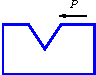
\includegraphics[width=0.3\linewidth]{..//Common/images/polydecomp_traverse.pdf} }%\\

%------------------------------------------------------------------------------------------------------------------------------------
\item 
Check if $P_i$ is a Reflex vertex $R$%&



\raisebox{-.9\height}{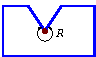
\includegraphics[width=0.3\linewidth]{..//Common/images/polydecomp_reflex.pdf} }%\\

%------------------------------------------------------------------------------------------------------------------------------------
\item 
Extend lines incident at $P_i$ (the line coming into $P_i$ and going out of $P_i$ ) till they intersect remaining of the Polygon, say at $Q_1$ and $Q_2$. Contour within $Q_1$ and $Q_2$ is called the $Range$. %&

\raisebox{-.9\height}{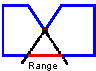
\includegraphics[width=0.3\linewidth]{..//Common/images/polydecomp_range.pdf} }%\\

%------------------------------------------------------------------------------------------------------------------------------------
\item 
If there are no $P_i$s within the $Range$ and if any of the $Range$ vertices are close to intersections, separate the triangle out. Else, create a new one at the middle of the contour. This newly created point  $Q_m$ is called Steiner point.  $RQ_m$ is the partition-chord to divide the polygon. %&

\raisebox{-.9\height}{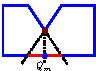
\includegraphics[width=0.3\linewidth]{..//Common/images/polydecomp_mid.pdf} }%\\

%------------------------------------------------------------------------------------------------------------------------------------
\item 
If there are a few vertices within the $Range$, choose the best one based on following priorities:
\begin{enumerate}
[noitemsep,topsep=2pt,parsep=2pt,partopsep=2pt,leftmargin=*]
\item Highest : Closest Reflex
\item Medium : Reflex 
\item Low : Closest 
\end{enumerate} 
%&
\added[remark={The pseudo-code under Algorithm 1 Polygon Decomposition.Clarify the meaning of "Make sure B is visible from R".  What happens when there is no visibility?}]{Make sure that point $Q_i$ is visible from the reflex point $R$. If it is not so, then this cut cannot be made. Choose the next best choice.}

\raisebox{-.9\height}{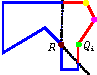
\includegraphics[width=0.3\linewidth]{..//Common/images/polydecomp_choice.pdf} }%\\

%------------------------------------------------------------------------------------------------------------------------------------
\item 
Once the vertex is chosen, say, $Q_i$, create a partition chord $RQ_i$ and divide the  polygon.% &

\raisebox{-.9\height}{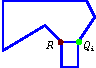
\includegraphics[width=0.3\linewidth]{..//Common/images/polydecomp_divide.pdf} } %\\


%\end{tabular}

%------------------------------------------------------------------------------------------------------------------------------------
\item 
Send individual sub-polygons to the same process recursively till there are no reflex vertices left. 

\item  
Identify polygons with more than 4 distinct (ignoring sub-segment overlapping chords) sides. Triangulate them with Constrained Delaunay Triangulation (CDT).

\raisebox{-.9\height}{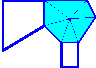
\includegraphics[width=0.31\linewidth]{..//Common/images/polydecomp_divide_all.pdf}} %\\

\added[remark={The second example section 3.1.2 steps. Complete the example until no mere reflex points remains. It would add to the understanding. It is difficult to understand all from the pseudo - code. }]{ CDT takes care of remaining areas of the polygon.}

%\end{list}
\end{enumerate}



\subsection{Improvements over Bayazit's algorithm}

\begin{tabular}[!h]{@{}p{0.7\linewidth} p{0.01\linewidth} p{0.35\linewidth}@{}}

\replaced[]{{\bf Algorithm \ref{alg1}} improves upon the Bayazit's algorithm \citep{Bayazit} in terms of expanding search to even include extreme vertices in the range, thereby giving minimal and elongated partitions. Midcurve is typically computed for a thin-elongated shape. This improvement results in the sub-polygons of necessary shape characteristics. If any incoming edge ($MR$) was hitting the end points of the test-line ($QN$) or was collinear, it ($Q$) was getting ignored in the existing algorithm \citep{Bayazit}. In that case the next closet vertex ($S$) was getting chosen. This was corrected in the proposed algorithm and the shorter cut ($RQ$) is done.} &&

\raisebox{-\height}{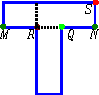
\includegraphics[width=0.8\linewidth]{..//Common/images/polydecomp_mine.pdf} }\\
\\
\end{tabular}

\begin{table}[!h]
\caption{Improvement over  Bayazit's \citep{Bayazit} partitioning algorithm}
\begin{tabular}[htb]{@{} p{0.31\linewidth} p{0.31\linewidth} p{0.31\linewidth}@{}}
\toprule

{\bf Shape } & {\bf Bayazit} & {\bf Proposed}\\
\midrule
%------------------------------------------------------------------------------------------------------------------------------------
%T &
\raisebox{0.08\height}{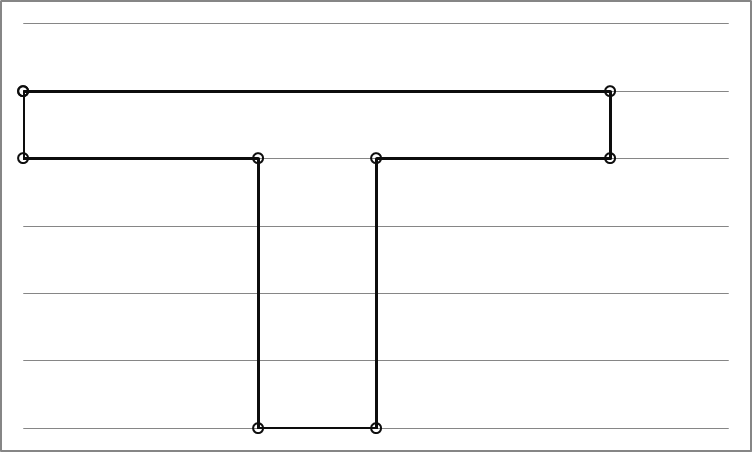
\includegraphics[width=0.98\linewidth]{..//Common/images/Ts.png}} &
\raisebox{0.08\height}{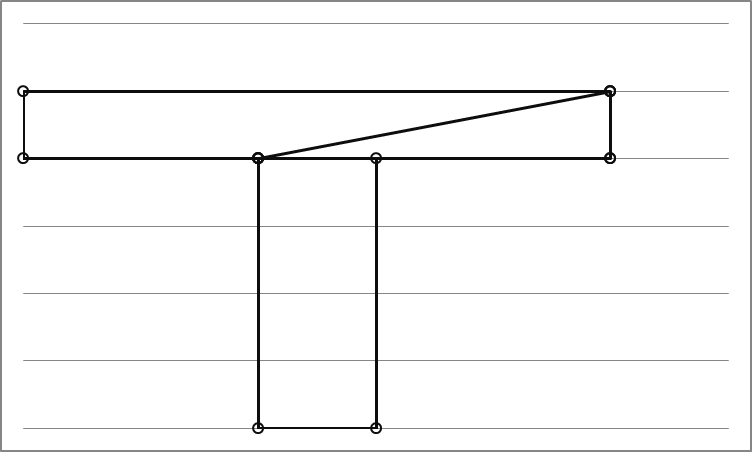
\includegraphics[width=0.98\linewidth]{..//Common/images/Tb.png}}&
\raisebox{0.08\height}{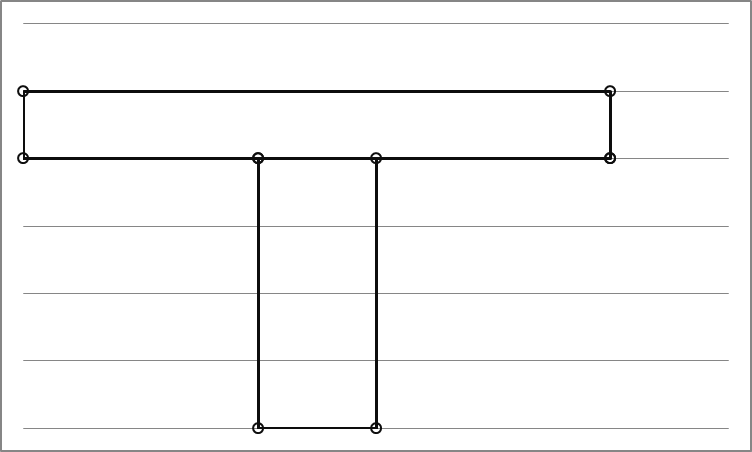
\includegraphics[width=0.98\linewidth]{..//Common/images/Tp.png}} \\


%------------------------------------------------------------------------------------------------------------------------------------
%Plus  &
\raisebox{0.08\height}{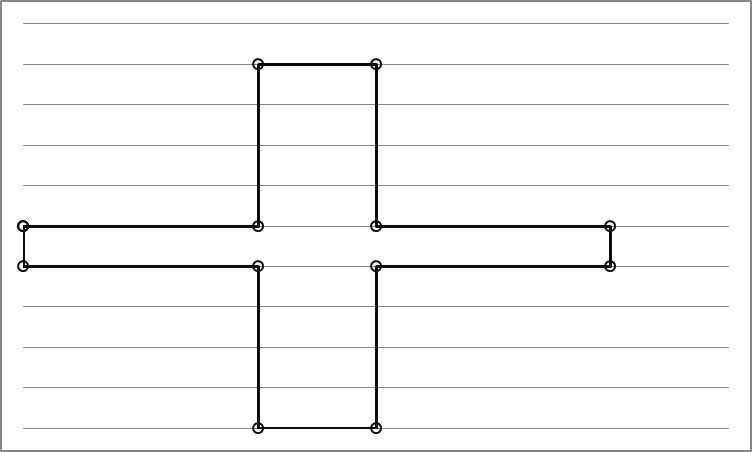
\includegraphics[width=0.98\linewidth]{..//Common/images/Pluss.png}} &
\raisebox{0.08\height}{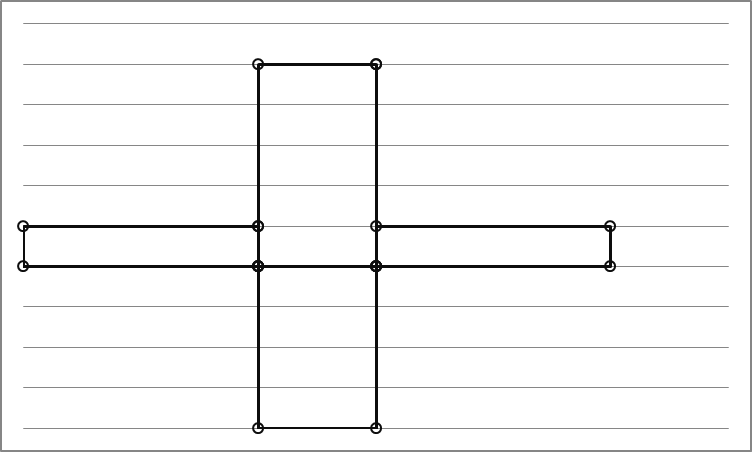
\includegraphics[width=0.98\linewidth]{..//Common/images/Plusb.png}}&
\raisebox{0.08\height}{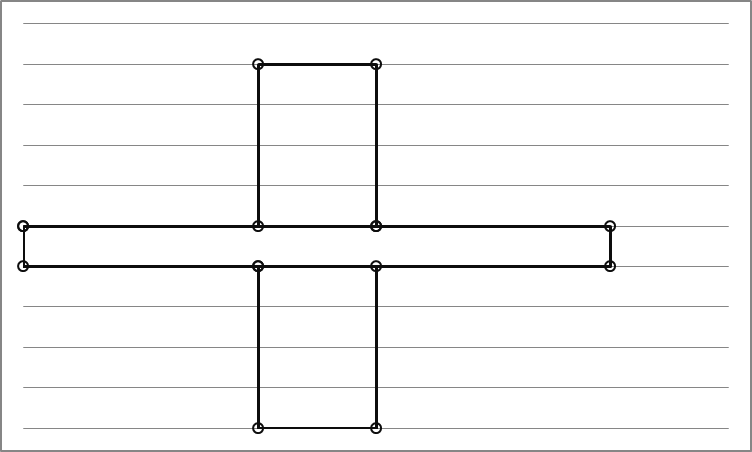
\includegraphics[width=0.98\linewidth]{..//Common/images/Plusp.png}} \\


%------------------------------------------------------------------------------------------------------------------------------------
%Star &
\raisebox{0.08\height}{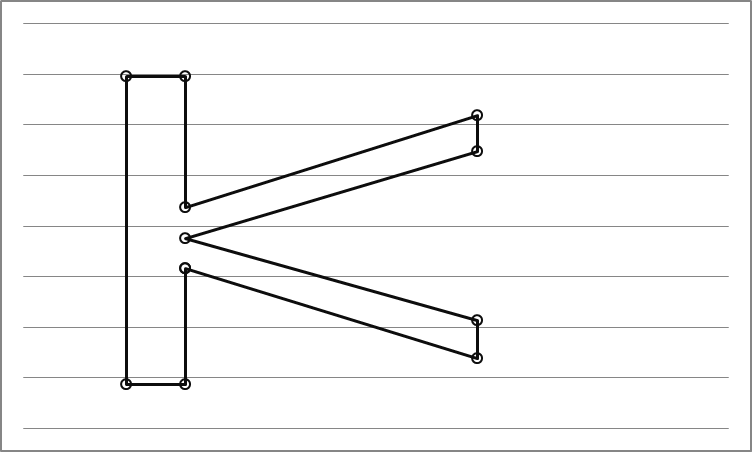
\includegraphics[width=0.98\linewidth]{..//Common/images/Ks.png}} &
\raisebox{0.08\height}{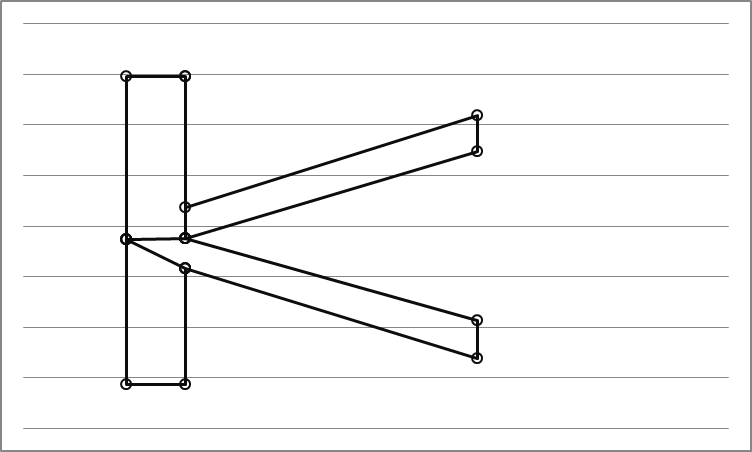
\includegraphics[width=0.98\linewidth]{..//Common/images/Kb.png}}&
\raisebox{0.08\height}{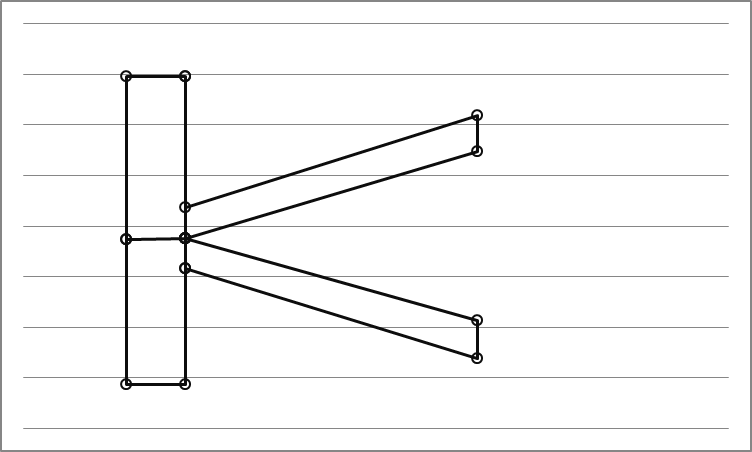
\includegraphics[width=0.98\linewidth]{..//Common/images/Kp.png}} \\

%------------------------------------------------------------------------------------------------------------------------------------
%Star &
\raisebox{0.08\height}{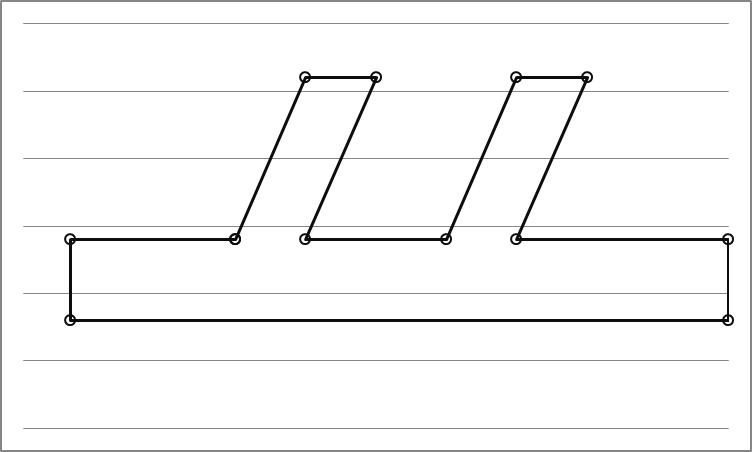
\includegraphics[width=0.98\linewidth]{..//Common/images/DoubleKs.png}} &
\raisebox{0.08\height}{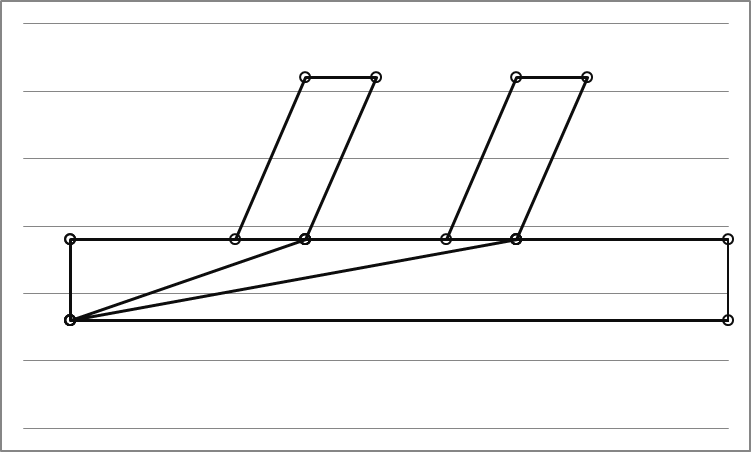
\includegraphics[width=0.98\linewidth]{..//Common/images/DoubleKb.png}}&
\raisebox{0.08\height}{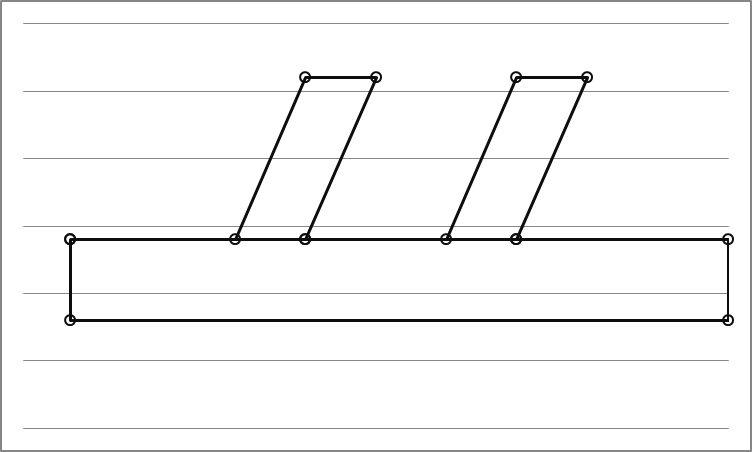
\includegraphics[width=0.98\linewidth]{..//Common/images/DoubleKp.png}} \\

\bottomrule
\end{tabular}
\label{PartitionComparision}
\end{table}

As the last step in the {\bf Algorithm \ref{alg1}} triangulates the remaining polygons, this algorithm guarantees presence of sub-polygons with 3 and 4 sides only. Further algorithms, like the one mentioned below {\bf Algorithm \ref{alg2}}, need to enumerate a case possible only with triangles and quadrilaterals, making it deterministic. {\bf Table \ref{PartitionComparision}} demonstrates improvements over Bayazit's \citep{Bayazit} algorithm with examples.  The resulting sub-polygons are sent for creating a connected midcurve.


\subsection{Midcurve Creation}

Decomposition helped getting the sub-polygons, which are of primitive shapes and which are easier for midcurve creation compared to the original-whole shape. 


\subsubsection{Preliminaries }

\begin{tabular}[h]{@{}p{0.6\linewidth} p{0.3\linewidth}@{}}
%\begin{figure} [h]
%	%\centering
%	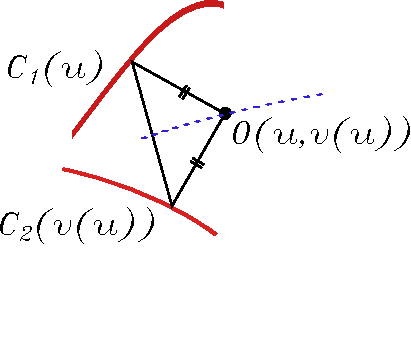
\includegraphics[width=0.5\linewidth]{..//Common/images/MidcurvesDefn.pdf}
%%	\vspace{-1cm}
%	\caption{Midcurve norm}
%	\label{figure_midcurve}
%\end{figure}

For the two curves $C_1(u)$ and $C_2(v(u))$, let there be a point $O(u_0, v(u_0))$ which is neither on the given curves, but is such that normals from both $C_1(u_0)$ and  $C_2(v(u_0))$  meet at $O$. Length of the normal denoted by $||C_1(u_0) - O(u_0, v(u_0))||$ in the neighborhood of $u_0$ is the shortest distance. 

 If, for all $u$ there exists a point $O(u, v(u))$ that is at equal (normal) distance from   $C_1(u)$ and $C_2(v(u))$, we say that curves  $C_1(u)$ and $C_2(v(u))$ are ideal-matched under the midcurve norm \citep{Elber1999}.%(Figure \ref{figure_midcurve})
&

\raisebox{-.9\height}{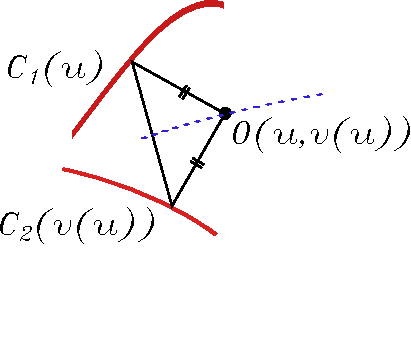
\includegraphics[width=1.5\linewidth]{..//Common/images/MidcurvesDefn.pdf}} \\
\end{tabular}

\begin{algorithm}
	\caption{Midcurve Creation}
	\label{alg2}
	\begin{algorithmic}
		\REQUIRE A list of partitioned 2D Planar polygons, each represented by a list of vertices in counter-clockwise direction
		\STATE Find internal-common edges called chords
		\STATE Iterate over all polygons and create chords at Full or Partial overlaps
		\WHILE{End of Polygons list has  not reached}
			\STATE Get the current polygon $P$
			\STATE Get chords that are part of $P$
			\STATE Look at the various combinations based on number of sides and number of chords
			\STATE Generate midcurve
			\STATE Assign midcurve on relevant side of the chord
		\ENDWHILE
		\STATE Extend chords that are not connected with other neighboring chords
	\end{algorithmic}
\end{algorithm}


\subsubsection{Steps}

\begin{tabular}[h]{@{}p{0.6\linewidth} p{0.03\linewidth} p{0.27\linewidth}@{}}
%\begin{enumerate}
%[noitemsep,topsep=2pt,parsep=2pt,partopsep=2pt,leftmargin=*]
%\begin{itemize}
%------------------------------------------------------------------------------------------------------------------------------------
%\item
Partitioning: Decompose polygons into  sub-polygons of primitive shapes using {\bf Algorithm \ref{alg1}}. Each additional edge inserted during the decomposition is called as the 'chord'. & &

\raisebox{-.9\height}{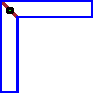
\includegraphics[width=0.8\linewidth]{..//Common/images/midcurve_polydecomp.pdf}} \\
\\

%------------------------------------------------------------------------------------------------------------------------------------
%\item
Generate midcurve for individual polygons taking chords into consideration. 'Thinness' is an important criterion in choosing midcurve for an individual shape. Midcurve is generated along longer-length and not across shorter-width. &&

\raisebox{-.9\height}{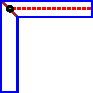
\includegraphics[width=0.8\linewidth]{..//Common/images/midcurve_polymid.pdf}} \\
\\

%------------------------------------------------------------------------------------------------------------------------------------
%\item 
In shapes like 'L', midcurves from both sub-polygons across the chord join together at a point, naturally. But in case of shapes like 'T', the horizontal midcurve does not connect with the common chord. In this case, one of the midcurves needs to be extended to join the other one. &&

\raisebox{-.9\height}{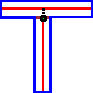
\includegraphics[width=0.8\linewidth]{..//Common/images/midcurve_extend.pdf}} \\
\\
%\end{itemize}
\end{tabular}
%\end{enumerate}
%\vspace{.1cm}

Each such shape can create its own midcurve based on number of sides and also where the cutting-chords lie on this individual shape. Tables \ref{Configurationst}, \ref{Configurationsp} have more details. A chord is a common interface-boundary shared between two sub-polygons. Each chord will have two sides owned by two different sub-polygons. Each sub-polygon needs to look at its own shape, slenderness and decide its own midcurve.

\begin{table}[!h]
\caption{Triangle cases of midcurve configuration}
\begin{tabular}[h]{@{}p{0.16\linewidth}@{} p{0.18\linewidth} @{}p{0.36\linewidth} p{0.15\linewidth}@{}} \toprule
{\bf Shape } & {\bf Chords }  & {\bf Rule} & {\bf Diagram}\\
\midrule

%------------------------------------------------------------------------------------------------------------------------------------
Triangle &
None&
No midcurve &
\raisebox{-.9\height}{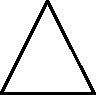
\includegraphics[width=0.5\linewidth]{..//Common/images/mids_t0.pdf} }\\

%------------------------------------------------------------------------------------------------------------------------------------
&
One &
Join midpoint of the shorter side &
\raisebox{-.9\height}{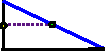
\includegraphics[width=0.5\linewidth]{..//Common/images/mids_t1_side.pdf} }\\

%------------------------------------------------------------------------------------------------------------------------------------
&
One &
Join opposite vertex if both the sides are of same length &
\raisebox{-.9\height}{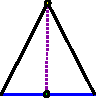
\includegraphics[width=0.5\linewidth]{..//Common/images/mids_t1.pdf} }\\

%------------------------------------------------------------------------------------------------------------------------------------
&
Two &
Join bisectors &
\raisebox{-.9\height}{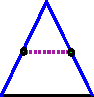
\includegraphics[width=0.5\linewidth]{..//Common/images/mids_t2.pdf} }\\

%------------------------------------------------------------------------------------------------------------------------------------
&
Three &
Join to centroid &
\raisebox{-.9\height}{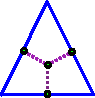
\includegraphics[width=0.5\linewidth]{..//Common/images/mids_t3.pdf} }\\

\bottomrule

\end{tabular}
\label{Configurationst}
\end{table}

\begin{table}[!h]
\caption{Polygon cases of midcurve configuration}
\begin{tabular}[h]{@{}p{0.13\linewidth} p{0.18\linewidth}  p{0.35\linewidth}  p{0.15\linewidth}@{}} \toprule

{\bf Shape } & {\bf Chords }  & {\bf Rule} & {\bf Diagram}\\
\midrule
%------------------------------------------------------------------------------------------------------------------------------------
Quad &
None&
Find the shortest side and create a midcurve in the direction average of both the adjacent sides &
\raisebox{-.9\height}{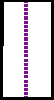
\includegraphics[width=0.5\linewidth]{..//Common/images/mids_q0.pdf} }\\

%------------------------------------------------------------------------------------------------------------------------------------
&
One (Shorter) &
Create a midcurve in the direction average of both the adjacent sides &
\raisebox{-.9\height}{
\includegraphics[width=0.5\linewidth]{..//Common/images/mids_q1s.pdf} }\\


%------------------------------------------------------------------------------------------------------------------------------------
&
One (Longer)&
None &
\raisebox{-.9\height}{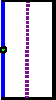
\includegraphics[width=0.5\linewidth]{..//Common/images/mids_q1l.pdf} }\\


%------------------------------------------------------------------------------------------------------------------------------------
&
Two (Opposite)&
Join midpoints &
\raisebox{-.9\height}{
\includegraphics[width=0.5\linewidth]{..//Common/images/mids_q2o.pdf} }\\


%------------------------------------------------------------------------------------------------------------------------------------
&
Two (Adjacent) &
Ignore the chord on the longer side and use the one-chord rule &
\raisebox{-.9\height}{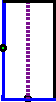
\includegraphics[width=0.5\linewidth]{..//Common/images/mids_q2a.pdf} }\\


%------------------------------------------------------------------------------------------------------------------------------------
&
Three &
Join to the centroid &
\raisebox{-.9\height}{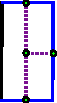
\includegraphics[width=0.5\linewidth]{..//Common/images/mids_q3.pdf} }\\


%------------------------------------------------------------------------------------------------------------------------------------
&
Four &
Join to the centroid &
\raisebox{-.9\height}{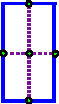
\includegraphics[width=0.5\linewidth]{..//Common/images/mids_q4.pdf} }\\

%\end{tabular}
%\label{Configurationsq}
%\end{table}
%
%\begin{table}[!h]
%\caption{Polygon cases of Midcurve configuration}
%\begin{tabular}[h]{|p{1cm} | p{1cm} | p{3cm} | p{1.2cm}|}
%\hline
%{\bf Shape } & {\bf Chords }  & {\bf Rule} & {\bf Diagram}\\
%\hline

%------------------------------------------------------------------------------------------------------------------------------------
Polygon &
None&
If thin, then CDT or CAT &
\raisebox{-.9\height}{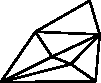
\includegraphics[width=0.5\linewidth]{..//Common/images/mids_p0.pdf} }\\

%------------------------------------------------------------------------------------------------------------------------------------
&
Any &
Join to the centroid &
\raisebox{-.9\height}{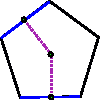
\includegraphics[width=0.5\linewidth]{..//Common/images/mids_pany.pdf} }\\
\bottomrule

\end{tabular}
\label{Configurationsp}
\end{table}

After creating individual midcurves, they all may or may not join at the chords. In case it does not join at any side of the chord, some extension has to be provided from the other side of that chord. Chords are processed to ignore the ones which have partial overlap with the sub-polygon sides or are collinear. This method gives cleaner (without branches) and a connected midcurve compared to the previously cited methods. A pseudo code for midcurve generation process is presented in Algorithm \ref{alg2}.

Many polygonal shapes can be broken down into $Regular$ and $Singular$ sub-shapes. $Singular$ regions correspond to the intersections, whereas $Regular$ regions are the remaining parts of the shapes \citep{Zou2001}.  Typical connection types \citep{You2002} and their midcurves are presented in Table \ref{table_ConnectionMidcurves}.

\begin{table}[!h]
\caption{Partitions and midcurve computation}
\begin{tabular}[h]{@{} p{0.31\linewidth} p{0.31\linewidth} p{0.31\linewidth}@{}}
\toprule
{\bf Shape } & {\bf Partitions} & {\bf Midcurve}\\
\midrule
%------------------------------------------------------------------------------------------------------------------------------------
%L &
\raisebox{-.9\height}{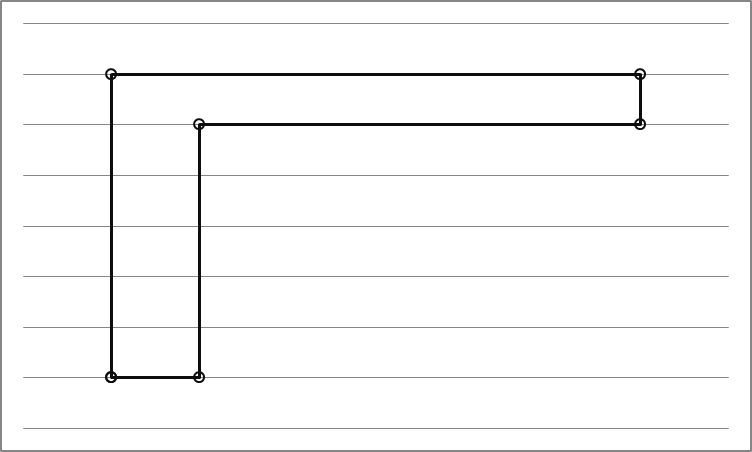
\includegraphics[width=0.98\linewidth]{..//Common/images/Ls.png}} &
\raisebox{-.9\height}{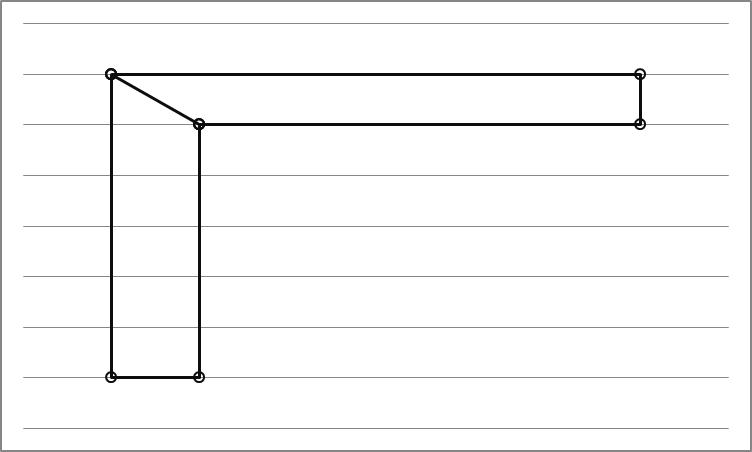
\includegraphics[width=0.98\linewidth]{..//Common/images/Lp.png}}&
\raisebox{-.9\height}{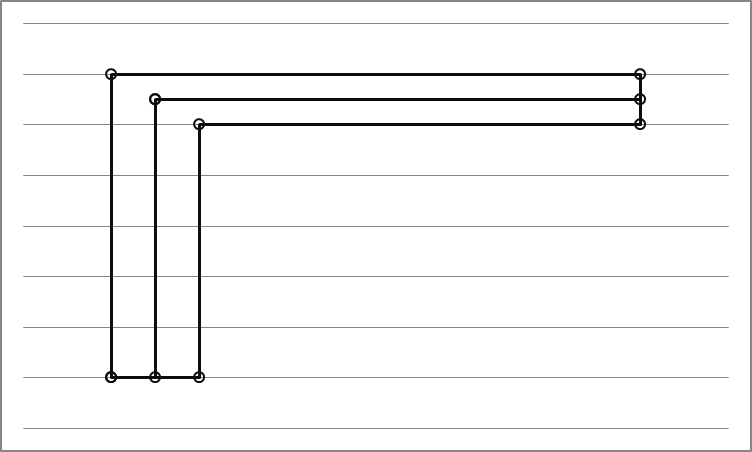
\includegraphics[width=0.98\linewidth]{..//Common/images/Lm.png}} \\

%------------------------------------------------------------------------------------------------------------------------------------
%Plus  &
\raisebox{-.9\height}{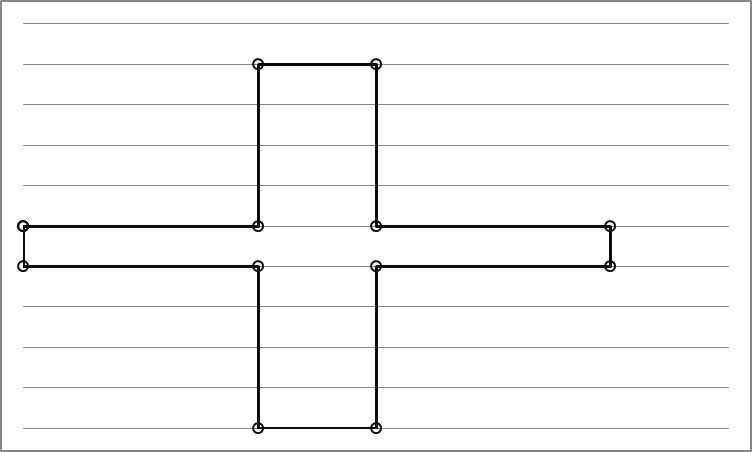
\includegraphics[width=0.98\linewidth]{..//Common/images/Pluss.png}} &
\raisebox{-.9\height}{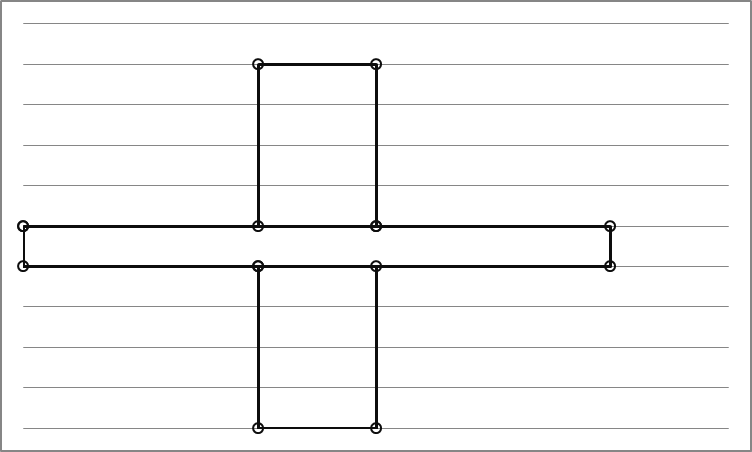
\includegraphics[width=0.98\linewidth]{..//Common/images/Plusp.png}}&
\raisebox{-.9\height}{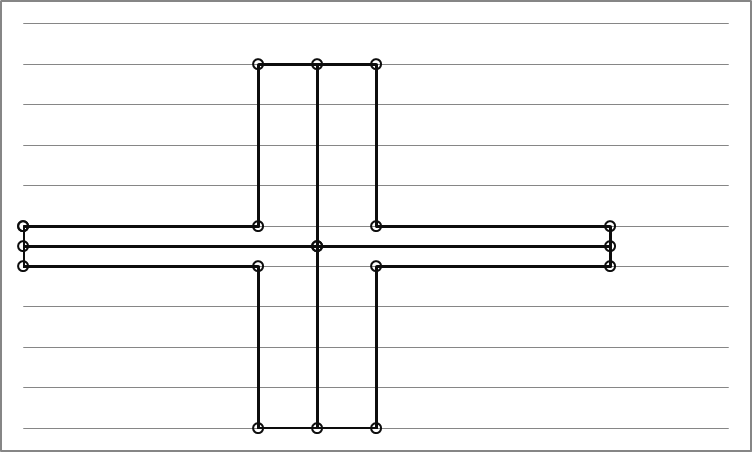
\includegraphics[width=0.98\linewidth]{..//Common/images/Plusm.png}} \\

%------------------------------------------------------------------------------------------------------------------------------------
%T &
\raisebox{-.9\height}{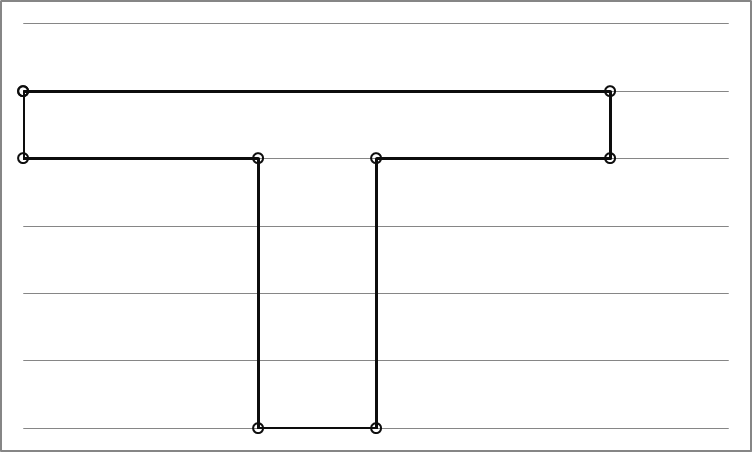
\includegraphics[width=0.98\linewidth]{..//Common/images/Ts.png}} &
\raisebox{-.9\height}{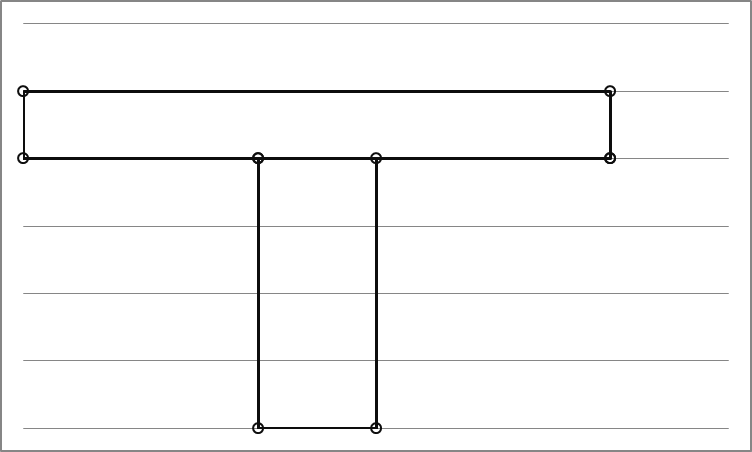
\includegraphics[width=0.98\linewidth]{..//Common/images/Tp.png}}&
\raisebox{-.9\height}{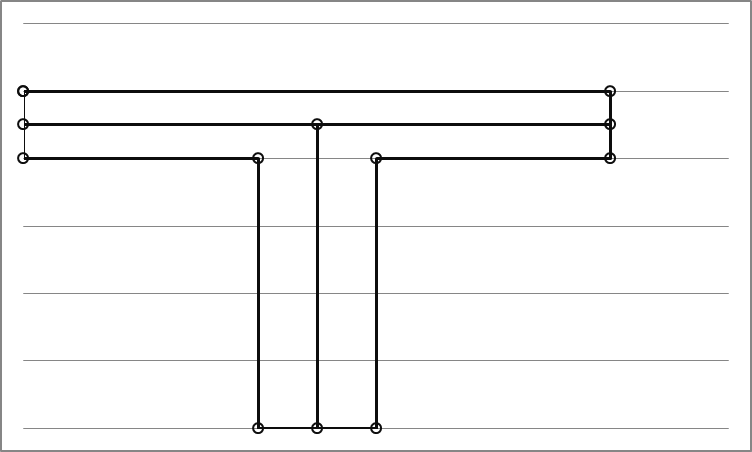
\includegraphics[width=0.98\linewidth]{..//Common/images/Tm.png}} \\

%------------------------------------------------------------------------------------------------------------------------------------
%K  &
\raisebox{-.9\height}{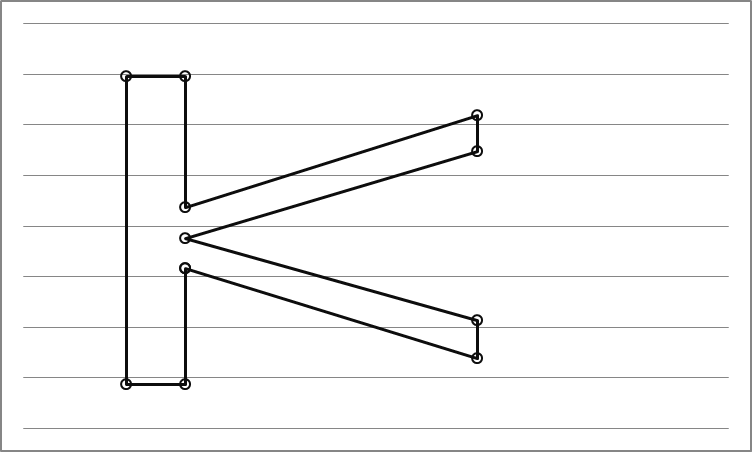
\includegraphics[width=0.98\linewidth]{..//Common/images/Ks.png}} &
\raisebox{-.9\height}{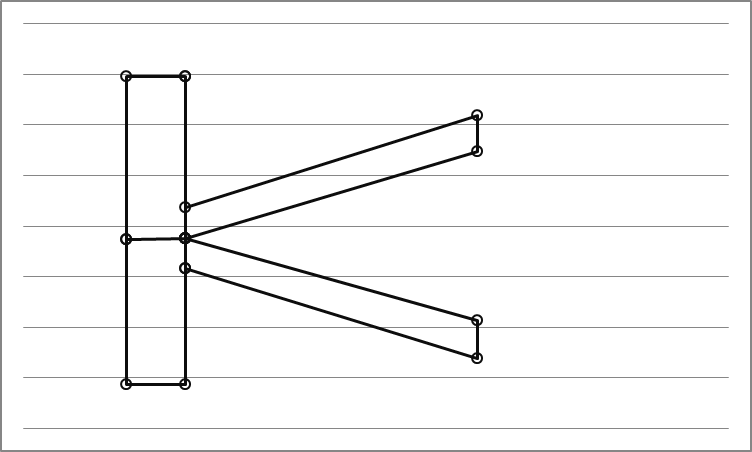
\includegraphics[width=0.98\linewidth]{..//Common/images/Kp.png}}&
\raisebox{-.9\height}{\includegraphics[width=0.98\linewidth]{..//Common/images/Km.png}} \\

%------------------------------------------------------------------------------------------------------------------------------------
%X &
\raisebox{-.9\height}{\includegraphics[width=0.98\linewidth]{..//Common/images/Xs.png}} &
\raisebox{-.9\height}{\includegraphics[width=0.98\linewidth]{..//Common/images/Xp.png}}&
\raisebox{-.9\height}{\includegraphics[width=0.98\linewidth]{..//Common/images/Xm.png}} \\

%------------------------------------------------------------------------------------------------------------------------------------
%V &
\raisebox{-.9\height}{\includegraphics[width=0.98\linewidth]{..//Common/images/Vs.png}} &
\raisebox{-.9\height}{\includegraphics[width=0.98\linewidth]{..//Common/images/Vp.png}}&
\raisebox{-.9\height}{\includegraphics[width=0.98\linewidth]{..//Common/images/Vm.png}} \\

%------------------------------------------------------------------------------------------------------------------------------------
%Y &
\raisebox{-.9\height}{\includegraphics[width=0.98\linewidth]{..//Common/images/Ys.png}} &
\raisebox{-.9\height}{\includegraphics[width=0.98\linewidth]{..//Common/images/Yp.png}}&
\raisebox{-.9\height}{\includegraphics[width=0.98\linewidth]{..//Common/images/Ym.png}} \\

\bottomrule
\end{tabular}
\label{table_ConnectionMidcurves}
\end{table}

\subsubsection{Limitations}

\added[remark={MAT can produce centerlines for such geometries with ease. The authors have not discussed test cases where their method could fail i.e. degenerate geometry.}]
{In practical scenarios, input geometry may not be clean. It may have degeneracies, which need to be addressed or corrected for a desired output. The current algorithm has following limitations even for a clean input:}
\begin{itemize}
%[noitemsep,topsep=2pt,parsep=2pt,partopsep=2pt,leftmargin=*]
\item \textbf{Faceting}: Even if the input is made up of curves, it is faceted to convert to a polygon. This approximation results in an approximation of the output as well. Thus, it does not give a true midcurve. It is possible to fit a curve through points of the midcurve-segments, but it may not match the expected result.
\item \textbf{Holes}: Input to the algorithm is in the form of a single ordered list of vertices, making a non-self-intersecting closed polygon.

\raisebox{-.9\height}{\includegraphics[width=0.3\linewidth]{..//Common/images/ProfileHoles.pdf}} 

%\vspace{2mm}

In case of holes, a connecting line is added to reach the internal holes to form a path, which does not traverse the given segments twice. If the number of holes are more, the situation becomes challenging to find the right connecting chords.
\end{itemize}


%\added[remark={MAT can produce centrelines for such geometries with ease. The authors have not discussed test cases where their method could fail i.e. degenerate geometry.}]
%{In practical scenarios, input geometry may not be clean, can have degeneracies etc, which need to be addressed-corrected before given algorithms to have predictable output. In special situation s like sudden change in thickness (\citep{Sheen2010}) limitations of Polygon Decomposition (Algorithm \ref{alg1}) show up in Midcurves (Algorithm \ref{alg2}). As shown below, although the partitioning is valid, it does not compute Midcurve as expected (even though there could be no clear expectation in this case, as well).}
%
%\begin{itemize}
%[noitemsep,topsep=2pt,parsep=2pt,partopsep=2pt,leftmargin=*]
%\item \textbf{Stepped Component}: There are conflicting expectation from such shape. If it has to mimic the profile then the Midcurve should have the {\em step}. But having a sudden change is sometimes not desirable, so a smooth blended curve could be the correct output.
%
%\raisebox{-.9\height}{\includegraphics[width=0.35\linewidth]{..//Common/images/steps.png}} 
%
%\item \textbf{Partitioning}: The {\em reflex} vertex finds opposite corner to form partitioning chord. 
%
%\raisebox{-.9\height}{\includegraphics[width=0.35\linewidth]{..//Common/images/stepp.png}}
%
%\item As Midcurves from both sides of the chord are to meet together, they are generated in (wrong) opposite direction.
%
%  \raisebox{-.9\height}{\includegraphics[width=0.35\linewidth]{..//Common/images/stepm.png}} 
%\end{itemize}
%
%\begin{table}[!h]
%\caption{Limitations}
%\begin{tabular}[h]{@{} p{0.31\linewidth} p{0.31\linewidth} p{0.31\linewidth}@{}}
%\toprule
%{\bf Shape} & {\bf Partitions} & {\bf Midcurves}\\
%\midrule
%\raisebox{-.9\height}{\includegraphics[scale=0.27]{..//Common/images/steps.png}} &
%\raisebox{-.9\height}{\includegraphics[scale=0.27]{..//Common/images/stepp.png}}&
%\raisebox{-.9\height}{\includegraphics[scale=0.27]{..//Common/images/stepm.png}} \\
%\bottomrule
%\end{tabular}
%\label{table_limitations}
%\end{table}

\subsubsection{Usage}
\added[remark={Discuss the intended use of your algorithms. Perhaps give examples from FEA}]{Midcurve has a wide variety of applications as it produces dimensionally reduced representation of the 2D shapes. Some representative usages are}:
\begin{itemize}
%[noitemsep,topsep=2pt,parsep=2pt,partopsep=2pt,leftmargin=*]
\item \textbf{Pattern Matching}: Instead of finding similarity between 2D profiles, it is easier to do the same with midcurve.

\item \textbf{Shape Retrieval}: For retrieving a particular 2D shape from the database, midcurve can be used as a signature, instead of string/tag based, thus making selection more deterministic.

\item \textbf{Midsurface}: For sweep based volumes, midsurface is nothing but  sweeping of the midcurve of the sketch.

%\vspace{2mm}

%\raisebox{-.9\height}{\includegraphics[width=0.75\linewidth]{..//Common/images/MidsurfSmallProfile.pdf}}

%\begin{figure} [h]
%	%\centering
%	\includegraphics[width=0.5\linewidth]{..//Common/images/MidcurvesDefn.pdf}
%%	\vspace{-1cm}
%	\caption{Midcurve norm}
%	\label{figure_midcurve}
%\end{figure}

\includegraphics[width=0.65\linewidth]{..//Common/images/MidsurfSmallProfile.pdf}

\end{itemize}


\section{Results}

The approach presented in this paper has been applied not just to the English alphabets but also to some typical real-life shapes. %(Table \ref{table_PracticalMidcurves}) . 

\added[remark={ Although the proposed method works for the class of geometries defined in the paper, most standard cross-sections could comprise complex splines/curves such as fillets. It is understood that for this technique to work, complex curves would have to be broken down to simpler line segments. This has been shown in
Table-6, examples 1 (glass profile) and 3 (Pinto's example). But it would be worthwhile to see how the mid-line from this method compares to those produced using MAT. The medial lines created using MAT will always lie along the true centerline i.e. load path in an engineering sense.}]{Curved profiles are faceted into polygons, making individual midcurve approximate. More accurate output can be achieved by lowering faceting-segments-size, but then the computation increases. Although MAT would give a {\em true centerline} output, it may have disadvantages such as extra branches, sensitivity to perturbations and so on.} 

Shapes mentioned below are taken from academic papers to demonstrate enhancements in the resultant midcurve. 

%
%\begin{table}[htb]
%\caption{Medials of real-life shapes}
%\begin{tabular}[htb]{@{}p{0.45\linewidth} p{0.35\linewidth}@{}}
%\toprule
%{\bf Type } & {\bf Midcurves}\\
%\midrule

\begin{enumerate}
%[noitemsep,topsep=2pt,parsep=2pt,partopsep=2pt,leftmargin=*]

\item
%------------------------------------------------------------------------------------------------------------------------------------
A glass profile was presented by Fischer et. al \citep{Elber1999}. They had to carry out an additional loop-elimination step to remove the self-intersections that occurred after the first offset operation. %&
\added[remark={By restricting the algorithm to constant thickness sections, the authors have chosen to deal with simple problems. The results shown in Table 6 for non symmetric sections i.e example 1 and 3 are not compared against true mid/medial lines. This limitation would prevent the implementation of the ideas proposed in this paper in an industry setting}]{This example has been particularly chosen for showcasing midcurve of a profile, having variable thickness. Midcurve is cleaner  than what MAT would generate, i.e. without branches at the corners.}

\vspace{1mm}

\includegraphics[angle=90, width=0.65\linewidth]{..//Common/images/Glassmc.png} %\\

\item
%------------------------------------------------------------------------------------------------------------------------------------
Profile presented by Ramanathan \citep{Ramanathan2004}. %&

\vspace{1mm}

\includegraphics[width=0.65\linewidth]{..//Common/images/DoubleKmc.png}%\\


\item
%------------------------------------------------------------------------------------------------------------------------------------
Pinto's \citep{Pinto2009} example of planar polygonal Horse profile. All the branches at the corners have been eliminated. %&

\vspace{1mm}

\includegraphics[width=0.65\linewidth]{..//Common/images/Horsemc.png}%\\

\item
%------------------------------------------------------------------------------------------------------------------------------------
Sheen et al \citep{Sheen2010} took  a typical plastic injection part profile. The approach presented here does not need any additional split operations. %&

\vspace{1mm}

\includegraphics[width=0.65\linewidth]{..//Common/images/Sheen1mc.png}%\\

\item 
Sheen et al \citep{Sheen2010} also took the following profile to compare midsurface creation in two commercial CAD software packages.  Both produced incorrect results.% &

\vspace{1mm}

\includegraphics[width=0.65\linewidth]{..//Common/images/Sheen2mc.png}%\\

\item
\added[remark={}]{Sheen et al \citep{Sheen2010}  presented a couple of cases where midcurve could be ambiguous, due to step-ramp kind of a profile. Having a gradual change in the midcurve is desirable in this situation. The following output given by the current algorithm looks appropriate:} %&

\vspace{1mm}

\includegraphics[width=0.65\linewidth]{..//Common/images/rampmc.png}%\\

\item
%------------------------------------------------------------------------------------------------------------------------------------
Woo \citep{Woo2013}  presented the following example to demonstrate when extensions are appropriate. Extension of the midcurve of the first vertical bar up to boundary is invalid whereas of the second vertical bar is valid. In the second case, corresponding extended part-faces are present. %&

\vspace{1mm}

\includegraphics[width=0.65\linewidth]{..//Common/images/Woomc.png}%\\

%\bottomrule
%
%\end{tabular}
%\label{table_PracticalMidcurves}
%\end{table}
\end{enumerate}

%\begin{itemize}[noitemsep,topsep=2pt,parsep=2pt,partopsep=2pt,label={},leftmargin=*]
%\begin{itemize}
%
%\item Glass profile was presented by Fischer \citep{Elber1999}. They had to carry-out loop-elimination step to eliminate the self-intersection that occurred after the first offset-like operation.
%
%\includegraphics[angle=90, width=\linewidth]{..//Common/images/Glassmc.png}
%
% Such post-processing is not required in the approach presented here.
%
%%------------------------------------------------------------------------------------------------------------------------------------
%\item Double K profile presented by Ramanathan \citep{Ramanathan2004}.
%
%\includegraphics[width=\linewidth]{..//Common/images/DoubleKmc.png}
%
%%------------------------------------------------------------------------------------------------------------------------------------
%\item  Pinto's \citep{Pinto2009} example of planar polygonal Horse profile. All the branches at the corners have been eliminated.
%
%\includegraphics[width=\linewidth]{..//Common/images/Horsemc.png}
%
%%------------------------------------------------------------------------------------------------------------------------------------
%\item Sheen et al \citep{Sheen2010} took  typical plastic injection part profile. Approach presented here does not need any additional split operations.
%
%\includegraphics[width=\linewidth]{..//Common/images/Sheen1mc.png}
%
%They took following profile to compare Midsurface creation in two commercial CAD software packages.  Both produced incorrect results. 
%
%\includegraphics[width=\linewidth]{..//Common/images/Sheen2mc.png}
%
%%------------------------------------------------------------------------------------------------------------------------------------
%\item  Woo \citep{Woo2013}  presented following example to demonstrate when extensions are appropriate. Extension of midcurves of the first vertical bar up-to boundary is invalid whereas of the second vertical bar is valid, as in the second case, corresponding extended part-faces are present.
%
%\includegraphics[width=\linewidth]{..//Common/images/Woomc.png}
%
%\end{itemize}

%
%\begin{table}[htb]
%\caption{Medials of real-life shapes}
%\begin{tabular}[htb]{@{}p{0.15\linewidth} p{0.75\linewidth}@{}}
%\toprule
%{\bf Type } & {\bf Midcurves}\\
%\midrule
%%------------------------------------------------------------------------------------------------------------------------------------
%Glass profile \citep{Elber1999} &
%%\raisebox{-.9\height}{\includegraphics[width=1.2\linewidth]{..//Common/images/Glasss.png}} &
%%\raisebox{-.9\height}{\includegraphics[width=0.98\linewidth]{..//Common/images/Glassp.png}}&
%\raisebox{-.9\height}{\includegraphics[width=\linewidth]{..//Common/images/Glassmc.png}} \\
%
%%------------------------------------------------------------------------------------------------------------------------------------
%Double K profile \citep{Ramanathan2004} &
%%\raisebox{-.9\height}{\includegraphics[width=1.2\linewidth]{..//Common/images/Glasss.png}} &
%%\raisebox{-.9\height}{\includegraphics[width=0.98\linewidth]{..//Common/images/Glassp.png}}&
%\raisebox{-.9\height}{\includegraphics[width=\linewidth]{..//Common/images/DoubleKmc.png}} \\
%
%%------------------------------------------------------------------------------------------------------------------------------------
%Horse profile  \citep{Pinto2009} &
%%\raisebox{-.9\height}{\includegraphics[width=1.2\linewidth]{..//Common/images/Horses.png}} &
%%\raisebox{-.9\height}{\includegraphics[width=0.98\linewidth]{..//Common/images/Horsep.png}}&
%\raisebox{-.9\height}{\includegraphics[width=\linewidth]{..//Common/images/Horsemc.png}} \\
%
%%------------------------------------------------------------------------------------------------------------------------------------
%Cover Part profile  \citep{Sheen2010} &
%%\raisebox{-.9\height}{\includegraphics[width=1.2\linewidth]{..//Common/images/Sheen1.png}} &
%%\raisebox{-.9\height}{\includegraphics[width=0.98\linewidth]{..//Common/images/Sheen1.png}}&
%\raisebox{-.9\height}{\includegraphics[width=\linewidth]{..//Common/images/Sheen1mc.png}} \\
%
%%------------------------------------------------------------------------------------------------------------------------------------
%Channel profile  \citep{Sheen2010} &
%%\raisebox{-.9\height}{\includegraphics[width=1.2\linewidth]{..//Common/images/Sheen1.png}} &
%%\raisebox{-.9\height}{\includegraphics[width=0.98\linewidth]{..//Common/images/Sheen1.png}}&
%\raisebox{-.9\height}{\includegraphics[width=\linewidth]{..//Common/images/Sheen2mc.png}} \\
%
%%------------------------------------------------------------------------------------------------------------------------------------
%Thick Thin profile  \citep{Woo2013} &
%%\raisebox{-.9\height}{\includegraphics[width=1.2\linewidth]{..//Common/images/Sheen1.png}} &
%%\raisebox{-.9\height}{\includegraphics[width=0.98\linewidth]{..//Common/images/Sheen1.png}}&
%\raisebox{-.9\height}{\includegraphics[width=\linewidth]{..//Common/images/Woomc.png}} \\
%
%%------------------------------------------------------------------------------------------------------------------------------------
%%Cross Channel profile &
%%%\raisebox{-.9\height}{\includegraphics[width=1.2\linewidth]{..//Common/images/Crosss.png}} &
%%%\raisebox{-.9\height}{\includegraphics[width=0.98\linewidth]{..//Common/images/Crossp.png}}&
%%\raisebox{-.9\height}{\includegraphics[width=\linewidth]{..//Common/images/Crossmc.png}} \\
%
%
%\bottomrule
%
%\end{tabular}
%\label{table_PracticalMidcurves}
%\end{table}
